\section{RANGE \& ENDURANCE}

\begin{whitebox}{}
    \begin{tabularx}{\columnwidth}{lclclc}
        $SR$ & $\unit{m.kg^{-1}}$ & Specific range\\
        $TSFC$ & $\unit{kg.(Ns)^{-1}}$ & Thrust specific fuel consumption\\
        $BSFC$ & $\unit{kg.(Nm)^{-1}}$ & Brake specific fuel consumption\\
        $E$ & $\unit{s}$ & Endurance\\
        $R$ & $\unit{m}$ & Range\\
        $W_1$ & $\unit{kg}$ & Start mass\\
        $W_2$ & $\unit{kg}$ & End mass\\
        $\eta_{prop}$ & $-$ & Propeller efficiency
    \end{tabularx}
\end{whitebox}

\resizebox{0.9\linewidth}{!}{
    \includegraphics[
    page = {20},
    trim = {4.0cm, 7.5cm, 5.0cm, 2.5cm}, % left, bottom, right, top
    clip
    ]{Lecture04.pdf}
}

\begin{highlightbox}{}
    \begin{align*}
        &SR=\frac{V}{\dot{m}_f}\\
        &TSFC=\frac{\dot{m}_f}{T}\\
        &BSFC=\frac{\dot{m}_f}{P}
    \end{align*}
\end{highlightbox}

\begin{whitebox}{\textbf{RANGE}}
    \begin{whitebox}{JETS}
        \blue{Conditions}
        \begin{itemize}
            \item $T=D$
        \end{itemize}
        
        \blue{Assumptions}
        \begin{itemize}
            \item $TSFC=$ const.
        \end{itemize}
        \mathbox{
            SR_{\max}=\left(\frac{V}{D}\right)_{\max}
        }
        \centering
        \resizebox{1.0\linewidth}{!}{
            \includegraphics[
            page = {21},
            trim = {0.0cm, 4.5cm, 12.0cm, 4.0cm}, % left, bottom, right, top
            clip
            ]{Lecture04.pdf}
        }
        \resizebox{0.9\linewidth}{!}{
            \includegraphics[
            page = {21},
            trim = {13.5cm, 4.5cm, 0.0cm, 4.0cm}, % left, bottom, right, top
            clip
            ]{Lecture04.pdf}
        }
    \end{whitebox}
    
    \begin{whitebox}{PROPS}
        \blue{Assumptions}
        \begin{itemize}
            \item $BSFC=$ const.
            \item $P=DV$
        \end{itemize}
        \mathbox{
            SR_{\max}=\left(\frac{V}{P}\right)_{\max}
        }
        \centering
        \resizebox{1.0\linewidth}{!}{
            \includegraphics[
            page = {22},
            trim = {0.0cm, 4.5cm, 12.0cm, 4.0cm}, % left, bottom, right, top
            clip
            ]{Lecture04.pdf}
        }
        \resizebox{0.9\linewidth}{!}{
            \includegraphics[
            page = {22},
            trim = {13.5cm, 4.5cm, 0.0cm, 4.0cm}, % left, bottom, right, top
            clip
            ]{Lecture04.pdf}
        }
    \end{whitebox}
\end{whitebox}

\begin{whitebox}{\textbf{ENDURANCE}}
    \begin{whitebox}{JETS}
        \blue{Assumptions}
        \begin{itemize}
            \item $T=D$ i.e. $V=$ const.
            \item $L=mg$
            \item $\sfrac{L}{D}=$ const. i.e. $c_L=$ const.
            \item $TSFC=$ const.
        \end{itemize}
    
        \mathbox{
            E=\frac{L}{gD}\frac{1}{TSFC}\ln\left(\frac{W_1}{W_2}\right)
        }
    \end{whitebox}
    
    \begin{whitebox}{PROPS}
        \blue{Assumptions}
        \begin{itemize}
            \item See above
            \item $P=P_m=\sfrac{DV}{\eta_{prop}}$
            \item $BSFC=$ const.
        \end{itemize}
        
        \mathbox{
            E=\frac{L}{gD}\frac{\eta_{prop}}{V}\frac{1}{BSFC}\ln\left(\frac{W_1}{W_2}\right)
        }
    \end{whitebox}
\end{whitebox}

\begin{whitebox}{\textbf{RANGE}}
    \mathbox{
            R=EV
    }
    \begin{whitebox}{LONG RANGE CRUISE}
        \resizebox{1.0\linewidth}{!}{
            \includegraphics[
            page = {28},
            trim = {2.5cm, 6.5cm, 2.5cm, 3.5cm}, % left, bottom, right, top
            clip
            ]{Lecture04.pdf}
        }
    \end{whitebox}
    \begin{whitebox}{PAYLOAD-RANGE CHART}
        \resizebox{1.0\linewidth}{!}{
            \includegraphics[
            page = {34},
            trim = {2.0cm, 3.0cm, 0.5cm, 3.0cm}, % left, bottom, right, top
            clip
            ]{Lecture04.pdf}
        }
    \end{whitebox}
\end{whitebox}
    



